\documentclass[12pt,a4paper]{article}
\usepackage[utf8]{inputenc}
\usepackage[T1]{fontenc}
\usepackage[spanish]{babel}
\usepackage{amsmath, amssymb, amsfonts}
\usepackage{geometry}
\usepackage{graphicx}
\usepackage{xcolor}
\usepackage{enumitem}
\usepackage{float}
\usepackage{booktabs}
\usepackage{array}
\usepackage[hidelinks]{hyperref}

\geometry{left=2.5cm, right=2.5cm, top=2.5cm, bottom=2.5cm}
\graphicspath{{imagenes/}}
\emergencystretch=3em

\newcommand{\dd}{\mathrm{d}}
\newcommand{\ee}{\mathrm{e}}

\title{\textbf{Oscilador de Morse Forzado y Amortiguado:\\ métodos numéricos, ruta al caos y sincronización}}
\author{Jesús David Vitola González\\[2pt] Física Computacional 2 -- Primer Examen Parcial, Punto 2}
\date{\today}

\begin{document}

\maketitle

\section{Fenomenología y pregunta física}

El potencial de Morse describe la vibración de una molécula diatómica mejor que el oscilador armónico, porque incluye dos rasgos que este no tiene: una pared repulsiva muy dura a distancias cortas y una región atractiva que se aplana a distancias largas, donde el enlace se rompe (disociación) \cite{morse1929}. Esa asimetría hace que el período de oscilación dependa de la energía (anarmonicidad) y que exista una energía máxima, $D$, por encima de la cual la partícula escapa.

El sistema estudiado es un oscilador de Morse al que se le añaden dos efectos: una fuerza de amortiguamiento viscoso $-\gamma v$ y una fuerza externa periódica $A\cos(\omega t)$. El amortiguamiento disipa energía, el forzamiento la inyecta, y su competencia con la no linealidad del potencial produce una dinámica rica: respuesta periódica, duplicación de período y comportamiento caótico.

Las preguntas físicas y numéricas que se abordan son:
\begin{enumerate}[label=\textbf{\arabic*.}]
    \item ¿Qué método de integración (Euler, Euler-Cromer, Runge-Kutta de orden 2, 3 y 4) ofrece la mejor relación entre precisión y costo para este sistema?
    \item ¿Cómo evoluciona el oscilador desde la condición inicial hasta su régimen estacionario?
    \item Al variar la amplitud $A$ del forzamiento, ¿cómo cambia la dinámica, y a qué amplitudes aparece el caos?
    \item Si se acoplan dos osciladores idénticos con condiciones iniciales distintas, ¿llegan a moverse al unísono?
\end{enumerate}

\section{Modelo matemático, variables y parámetros}

\subsection{Ecuación de movimiento}

Sea $x$ la posición (elongación del enlace), $v=\dot x$ la velocidad y $m$ la masa reducida. El potencial de Morse es
\begin{equation}
    P(x) = D\left(1-\ee^{-a(x-x_e)}\right)^{2},
    \label{eq:morse}
\end{equation}
donde $D$ es la energía de disociación, $a$ controla el ancho del pozo y $x_e$ es la posición de equilibrio. La fuerza conservativa es
\begin{equation}
    F_M(x) = -\frac{\dd P}{\dd x} = -2Da\left(\ee^{-a(x-x_e)}-\ee^{-2a(x-x_e)}\right),
\end{equation}
y la ecuación de movimiento completa, que es la que implementa el programa, es
\begin{equation}
    m\ddot x = -2Da\left(\ee^{-a(x-x_e)}-\ee^{-2a(x-x_e)}\right) - \gamma\,\dot x + A\cos(\omega t).
    \label{eq:mov}
\end{equation}
Se resuelve como sistema de primer orden en $(x,v)$:
\begin{equation}
    \dot x = v, \qquad \dot v = \frac{1}{m}\Big[F_M(x) - \gamma v + A\cos(\omega t)\Big].
\end{equation}

\subsection{Propiedades útiles}

\paragraph{Frecuencia de pequeñas oscilaciones.} Como $P''(x_e)=2Da^{2}$, cerca del equilibrio $\omega_0 = a\sqrt{2D/m}$.

\paragraph{Caso conservativo ($\gamma=0$, $A=0$).} La energía $E=\tfrac12 mv^{2}+P(x)$ se conserva. Para el potencial de Morse, el movimiento ligado ($0<E<D$) es periódico con frecuencia
\begin{equation}
    \omega(E) = \omega_0\sqrt{1-\frac{E}{D}},
    \label{eq:omegaE}
\end{equation}
de modo que el período crece con la energía y diverge cuando $E\to D$. Los puntos de retorno satisfacen $P(x)=E$, es decir, $x_\pm = x_e - \tfrac1a\ln\!\big(1\mp\sqrt{E/D}\big)$. Estos resultados exactos sirven para validar el código.

\paragraph{Balance de energía.} Con amortiguamiento y forzamiento,
\begin{equation}
    \frac{\dd E}{\dd t} = -\gamma v^{2} + A v\cos(\omega t),
\end{equation}
por lo que $E(t)$ ya no es constante (el programa la registra como diagnóstico, no como invariante).

\paragraph{Contracción del espacio de fase.} La divergencia del campo vectorial es $\partial\dot v/\partial v=-\gamma/m$, constante. Como el sistema es no autónomo, el espacio de fase efectivo es $(x,v,t)$, donde la dirección $t$ tiene exponente de Lyapunov nulo; por tanto, la suma de los dos exponentes restantes es $-\gamma/m$.

\subsection{Dos osciladores acoplados}

Para estudiar sincronización se acoplan dos osciladores idénticos con un resorte difusivo de constante $\kappa$:
\begin{align}
    m\ddot x_1 &= F_M(x_1) - \gamma\dot x_1 + A\cos(\omega t) + \kappa\,(x_2-x_1),\\
    m\ddot x_2 &= F_M(x_2) - \gamma\dot x_2 + A\cos(\omega t) + \kappa\,(x_1-x_2).
\end{align}
La medida de sincronización es el error $e(t)=|x_1(t)-x_2(t)|$.

\subsection{Diagnósticos de caos}

\paragraph{Sección de Poincaré estroboscópica.} Con período de forzamiento $T=2\pi/\omega$, se registra el estado en $t=nT$. Si la respuesta es periódica de período $T$ aparece un único punto; de período $2T$, dos puntos; y en régimen caótico, una nube de puntos.

\paragraph{Mayor exponente de Lyapunov.} Se sigue una trayectoria de referencia y otra perturbada, inicialmente separada una distancia $d_0$ en el espacio de fase $(x,v)$. Tras cada período se mide la distancia $d_1$, se acumula $\ln(d_1/d_0)$ y se renormaliza la separación a $d_0$ (método de Benettin \cite{benettin1980}):
\begin{equation}
    \lambda_{\max} \approx \frac{1}{N_p\,T}\sum_{k=1}^{N_p}\ln\frac{d_1^{(k)}}{d_0}.
\end{equation}
Un valor $\lambda_{\max}>0$ indica sensibilidad a las condiciones iniciales (caos); $\lambda_{\max}<0$, órbita periódica estable.

\subsection{Parámetros utilizados}

La Tabla~\ref{tab:param} resume los parámetros de cada conjunto de corridas. Todos los casos usan $x_e=0$ y $m=1$.

\begin{table}[H]
\centering
\footnotesize
\setlength{\tabcolsep}{3pt}
\begin{tabular}{@{}lcccccccc@{}}
\toprule
Corrida & $D$ & $a$ & $\gamma$ & $A$ & $\omega$ & $x_0$ & $v_0$ & Pasos\\
\midrule
Caso conservativo & 2 & 1.1 & 0 & 0 & -- & $-0.5$ & 0 & $dt=0.01$, $t_{\max}=41$\\
Experimentos 2a--2d & 5 & 1 & 0.2 & 2 & 2 & 0.5 & 0 & $dt=0.01$, $t_{\max}=40$\\
Bifurcación y Lyapunov & 5 & 1 & 0.5 & 1.5--4 & 2.6 & 0.5 & 0 & $dt=T/1000$\\
Osciladores acoplados & 5 & 1 & 0.5 & 3 & 2.6 & 0.5 / 0.501 & 0 / 0.5 & $dt=0.01$, $t_{\max}=80$\\
\bottomrule
\end{tabular}
\caption{Parámetros de las corridas. En los osciladores acoplados se usó $\kappa=1.5$, y las condiciones iniciales se indican como oscilador 1 / oscilador 2. Para los experimentos con $D=5$, $a=1$, $m=1$ se tiene $\omega_0=a\sqrt{2D/m}\approx 3.16$.}
\label{tab:param}
\end{table}

\section{Método computacional y justificación}

\subsection{Integradores}

Todos los esquemas avanzan el estado $(x,v)$ un paso $\Delta t$. Sea $\mathbf{y}=(x,v)$ y $\dot{\mathbf y}=\mathbf{f}(t,\mathbf{y})$ el campo definido por la ecuación de movimiento.

\begin{itemize}
    \item \textbf{Euler} (orden 1): $x_{n+1}=x_n+\Delta t\,v_n$, $\;v_{n+1}=v_n+\Delta t\,a_n$. La aceleración $a_n$ se evalúa con el estado anterior, de modo que $x$ y $v$ se actualizan con el mismo punto.
    \item \textbf{Euler-Cromer} (orden 1): primero $v_{n+1}=v_n+\Delta t\,a_n$ y luego $x_{n+1}=x_n+\Delta t\,v_{n+1}$. Es la variante semi-implícita simpléctica para sistemas conservativos \cite{cromer1981}.
    \item \textbf{RK2, punto medio} (orden 2): una evaluación en $\mathbf y_n$ y otra en el punto medio, $\mathbf y_{n+1}=\mathbf y_n+\Delta t\,\mathbf f\!\left(t_n+\tfrac{\Delta t}{2},\,\mathbf y_n+\tfrac{\Delta t}{2}\mathbf k_1\right)$.
    \item \textbf{RK3, de Kutta} (orden 3): $\mathbf k_1=\mathbf f(t_n,\mathbf y_n)$, $\mathbf k_2=\mathbf f(t_n+\tfrac{\Delta t}{2},\mathbf y_n+\tfrac{\Delta t}{2}\mathbf k_1)$, $\mathbf k_3=\mathbf f(t_n+\Delta t,\mathbf y_n-\Delta t\,\mathbf k_1+2\Delta t\,\mathbf k_2)$ y $\mathbf y_{n+1}=\mathbf y_n+\tfrac{\Delta t}{6}(\mathbf k_1+4\mathbf k_2+\mathbf k_3)$.
    \item \textbf{RK4 clásico} (orden 4): $\mathbf y_{n+1}=\mathbf y_n+\tfrac{\Delta t}{6}(\mathbf k_1+2\mathbf k_2+2\mathbf k_3+\mathbf k_4)$, con cuatro evaluaciones de $\mathbf f$ por paso \cite{press2007}.
\end{itemize}

\begin{table}[H]
\centering
\begin{tabular}{@{}lcc@{}}
\toprule
Método & Orden teórico & Evaluaciones de $\mathbf f$ por paso\\
\midrule
Euler & 1 & 1\\
Euler-Cromer & 1 & 1\\
RK2 & 2 & 2\\
RK3 & 3 & 3\\
RK4 & 4 & 4\\
\bottomrule
\end{tabular}
\caption{Métodos implementados.}
\end{table}

\subsection{Justificación}

\begin{itemize}
    \item El sistema forzado y amortiguado no es hamiltoniano, así que la propiedad simpléctica de Euler-Cromer no es una ventaja garantizada. Por eso se compara con los métodos de Runge-Kutta en lugar de asumirla.
    \item Se eligió RK4 para las corridas de física (bifurcación, Lyapunov, régimen estacionario y osciladores acoplados) porque, como se verá en la sección de resultados, su error es varios órdenes de magnitud menor que el de los demás métodos a igual $\Delta t$. En el caos, un error de integración pequeño importa más, porque cualquier perturbación se amplifica exponencialmente con $\lambda_{\max}>0$.
    \item El tiempo se calcula como $t=i\,\Delta t$ y no acumulando $t\mathrel{+}=\Delta t$, para no arrastrar error de redondeo dentro de $\cos(\omega t)$ en corridas largas.
    \item En la sección de Poincaré se toma $\Delta t=T/1000$, de modo que cada período contiene un número entero de pasos y el muestreo cae exactamente en $t=nT$.
    \item Se considera que el enlace se rompió si $x>15$ (umbral de disociación), y esa amplitud se omite en el barrido.
\end{itemize}

\section{Arquitectura del programa}

El código está escrito en C++ orientado a objetos. La clase \texttt{Osc\_Morse\_Forzado} encapsula el estado del oscilador (posición, velocidad y energía potencial) y los cinco integradores:

\begin{itemize}
    \item \texttt{Inicie(x0, v0, D, a, xe)}: fija el estado inicial y calcula $P(x_0)$.
    \item \texttt{calcularAceleracion(...)}: evalúa $\dot v$ según la ecuación~\eqref{eq:mov}.
    \item \texttt{calcularPotencial(...)}: actualiza $P(x)$ con la ecuación~\eqref{eq:morse}.
    \item \texttt{MuevaseEuler}, \texttt{MuevaseEulerCromer}, \texttt{MuevaseRK2}, \texttt{MuevaseRK3}, \texttt{MuevaseRK4}: avanzan un paso.
    \item \texttt{GetEnergia(m)}: devuelve $E=\tfrac12 mv^{2}+P$.
    \item \texttt{generarScriptsGnuplot()}: escribe y ejecuta los scripts de gnuplot de la simulación principal.
\end{itemize}

Los demás archivos usan esa clase:

\begin{table}[H]
\centering
\small
\begin{tabular}{@{}lp{10.5cm}@{}}
\toprule
Archivo & Función\\
\midrule
\texttt{punto2.cpp} & Función \texttt{ejecutarPunto2()}: pide los datos por teclado, elige simulación simple o acoplada, y escribe \texttt{trayectoria.dat}.\\
\texttt{acoplados.cpp} & \texttt{ejecutarAcoplados()}: integra dos osciladores con RK4 simultáneo y guarda las ocho columnas $t,x_1,v_1,P_1,x_2,v_2,P_2,e$.\\
\texttt{experimentos.cpp} & Programa independiente con cuatro etapas: convergencia, costo, comparación de trayectorias y régimen estacionario.\\
\texttt{bifurcacion.cpp} & Programa independiente: diagrama de bifurcación (Poincaré) y exponente de Lyapunov.\\
\bottomrule
\end{tabular}
\caption{Organización del código del Punto 2.}
\end{table}

\paragraph{Ejecución.} Desde la raíz del proyecto, la opción 2 del menú (\texttt{make run}) lanza \texttt{ejecutarPunto2()}. Los dos programas de experimentos se ejecutan con \texttt{make exp2} y \texttt{make bif2}. Todos escriben sus datos en \texttt{2.MorseForzado/results/datos/} y generan las figuras con gnuplot en \texttt{results/figuras/}. El Punto 2 es determinista: no usa números aleatorios.

\section{Experimentos computacionales realizados}

\begin{description}[leftmargin=!,labelwidth=2.2cm,style=nextline]
    \item[Validación (caso conservativo).] Con $\gamma=A=0$ se integra con RK4 y se compara con las expresiones exactas: conservación de $E$, período~\eqref{eq:omegaE} y puntos de retorno.
    \item[2a. Convergencia.] Se mide $|x(t_{\max})-x_{\mathrm{ref}}|$ para $\Delta t\in\{0.02,\,0.01,\,0.005,\,0.0025,\,0.00125\}$ y los cinco métodos. La referencia $x_{\mathrm{ref}}$ es RK4 con $\Delta t=5\times10^{-4}$. Con los dos pasos más finos se calcula el orden observado $p=\log_2\!\big[e(\Delta t)/e(\Delta t/2)\big]$.
    \item[2b. Costo vs.\ precisión.] Para cada método se mide el tiempo de cómputo con $\Delta t=5\times10^{-4}$ y el error final con $\Delta t=0.01$.
    \item[2c. Comparación de trayectorias.] Se integra con los cinco métodos ($\Delta t=0.01$, $t_{\max}=40$) y se calcula $|x(t)-x_{\mathrm{ref}}(t)|$ en todo el intervalo.
    \item[2d. Transitorio y régimen estacionario.] RK4 con $\Delta t=0.005$ hasta $t=100$; se grafican $x(t)$, $E(t)$ y el espacio de fase.
    \item[2e. Bifurcación y Lyapunov.] Barrido de $A$ de 1.5 a 4.0 en pasos de 0.02, con $\gamma=0.5$ y $\omega=2.6$. Para cada $A$ se descartan 200 períodos de transitorio, se registran 100 puntos de Poincaré y, para $\lambda_{\max}$, se promedia sobre 300 períodos con $d_0=10^{-8}$. Cada amplitud arranca de $(x_0,v_0)=(0.5,0)$.
    \item[2f. Osciladores acoplados.] RK4 simultáneo con $\kappa=1.5$ hasta $t=80$, partiendo de condiciones iniciales distintas.
\end{description}

\section{Resultados}

\subsection{Validación con el caso conservativo}

Con $D=2$, $a=1.1$, $m=1$, $x_0=-0.5$ y $v_0=0$, la energía inicial es $E_0=P(x_0)=1.07532$. Integrando con RK4 ($\Delta t=0.01$, $t\in[0,41)$) la energía se mantiene en $1.07532$ durante toda la corrida y el error relativo $(E-E_0)/E_0$ es cero a seis decimales (Figura~\ref{fig:energia}).

\begin{table}[H]
\centering
\begin{tabular}{@{}lcc@{}}
\toprule
Magnitud & Teoría & Simulación\\
\midrule
Período & $2\pi/\omega(E_0)=4.200$ & $4.20$\\
Retorno izquierdo $x_-$ & $-0.5$ & $-0.5$\\
Retorno derecho $x_+$ & $1.2013$ & $1.2013$\\
Velocidad máxima $\sqrt{2E_0/m}$ & $1.4665$ & $1.4665$\\
\bottomrule
\end{tabular}
\caption{Comparación entre las expresiones exactas del caso conservativo y la simulación. Con $\omega_0=a\sqrt{2D/m}=2.2$ y $E_0/D=0.5377$ se obtiene $\omega(E_0)=1.4959$. El período numérico se estimó de nueve oscilaciones entre máximos de $x$, con resolución $\Delta t=0.01$.}
\label{tab:validacion}
\end{table}

El espacio de fase es una curva cerrada asimétrica (Figura~\ref{fig:fase}), con $x$ entre $-0.5$ y $1.2$: el lado izquierdo, de pared dura, queda más comprimido que el derecho.

\begin{figure}[H]
    \centering
    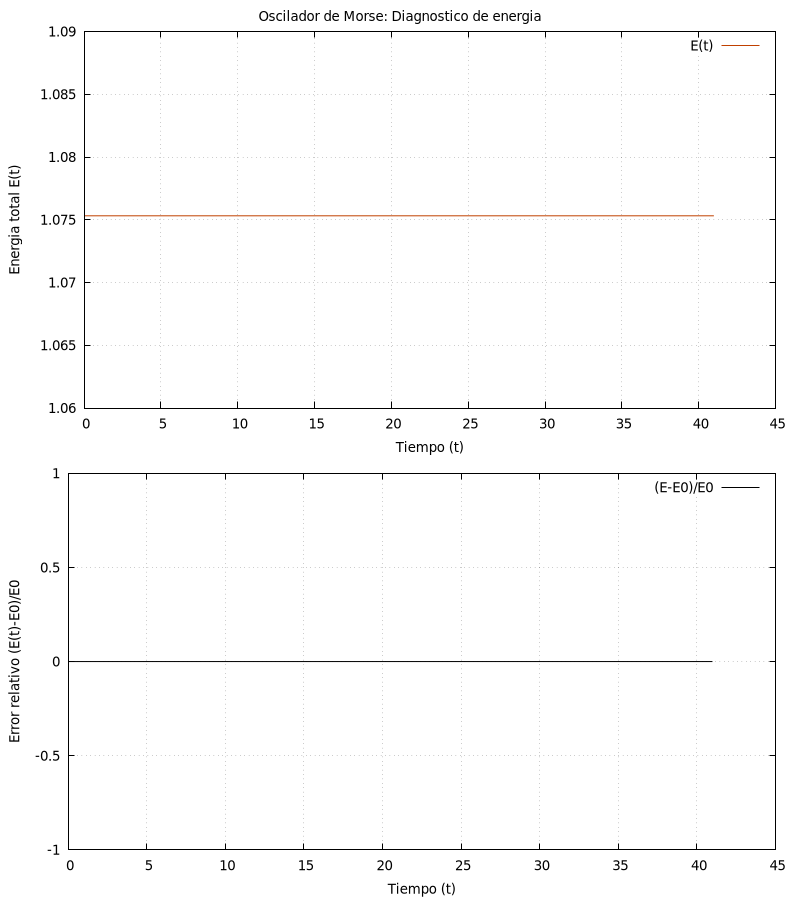
\includegraphics[width=0.62\textwidth]{energia.png}
    \caption{Caso conservativo: $E(t)$ constante y error relativo nulo con RK4.}
    \label{fig:energia}
\end{figure}

\begin{figure}[H]
    \centering
    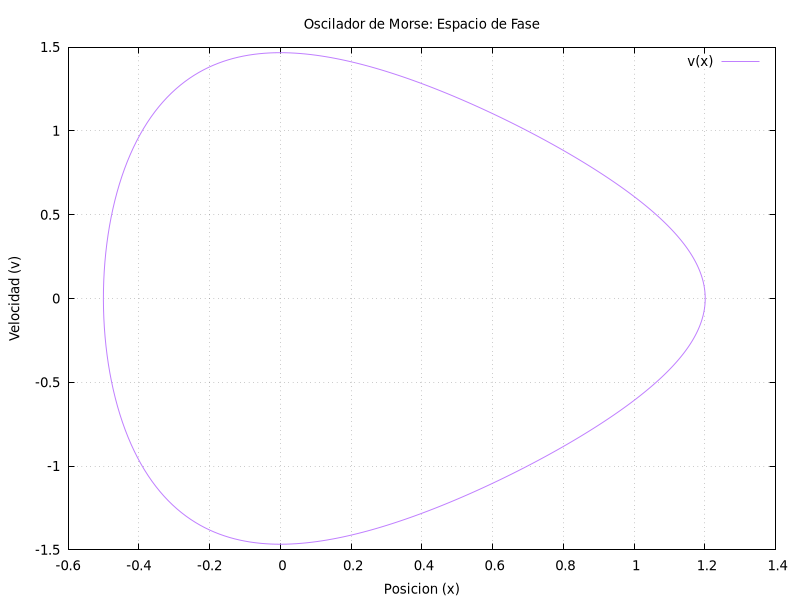
\includegraphics[width=0.58\textwidth]{espacio_fase.png}
    \caption{Espacio de fase del caso conservativo: órbita cerrada y asimétrica.}
    \label{fig:fase}
\end{figure}

\subsection{Convergencia y orden de los métodos (2a)}

\begin{table}[H]
\centering
\small
\begin{tabular}{@{}lccccc@{}}
\toprule
$\Delta t$ & Euler & Euler-Cromer & RK2 & RK3 & RK4\\
\midrule
$2\times10^{-2}$ & $3.59\times10^{-2}$ & $2.09\times10^{-4}$ & $3.40\times10^{-4}$ & $2.13\times10^{-5}$ & $9.82\times10^{-8}$\\
$1\times10^{-2}$ & $1.51\times10^{-2}$ & $8.17\times10^{-5}$ & $7.69\times10^{-5}$ & $2.69\times10^{-6}$ & $5.18\times10^{-9}$\\
$5\times10^{-3}$ & $8.56\times10^{-3}$ & $3.49\times10^{-5}$ & $1.82\times10^{-5}$ & $3.38\times10^{-7}$ & $2.93\times10^{-10}$\\
$2.5\times10^{-3}$ & $4.35\times10^{-3}$ & $1.59\times10^{-5}$ & $4.42\times10^{-6}$ & $4.23\times10^{-8}$ & $1.74\times10^{-11}$\\
$1.25\times10^{-3}$ & $2.18\times10^{-3}$ & $7.56\times10^{-6}$ & $1.09\times10^{-6}$ & $5.30\times10^{-9}$ & $1.03\times10^{-12}$\\
\bottomrule
\end{tabular}
\caption{Error $|x(t_{\max})-x_{\mathrm{ref}}|$ con $t_{\max}=40$ para cada método y paso.}
\label{tab:conv}
\end{table}

\begin{table}[H]
\centering
\begin{tabular}{@{}lccccc@{}}
\toprule
 & Euler & Euler-Cromer & RK2 & RK3 & RK4\\
\midrule
Orden teórico & 1 & 1 & 2 & 3 & 4\\
Orden observado $p$ & 0.99 & 1.07 & 2.02 & 3.00 & 4.07\\
\bottomrule
\end{tabular}
\caption{Orden observado con los dos pasos más finos ($2.5\times10^{-3}$ y $1.25\times10^{-3}$).}
\label{tab:orden}
\end{table}

\begin{figure}[H]
    \centering
    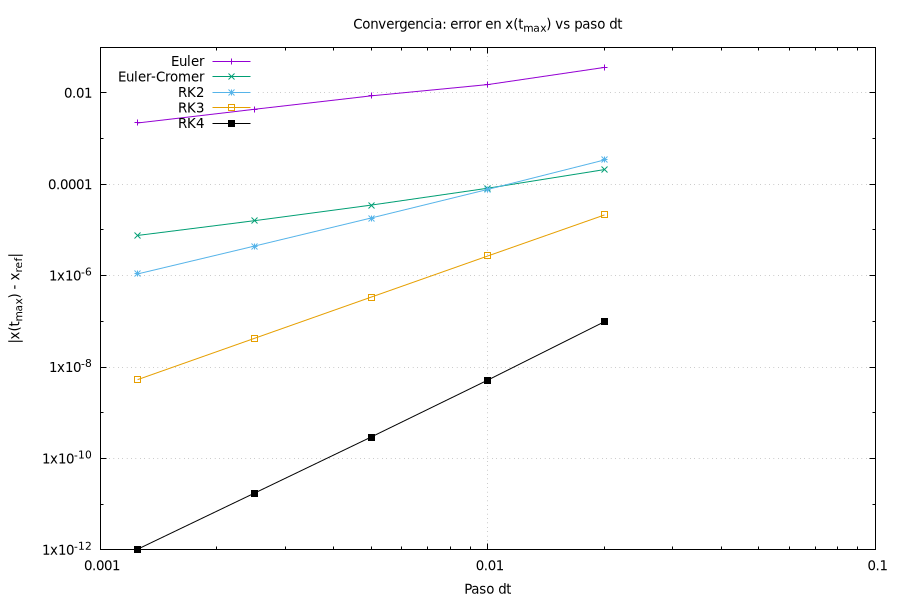
\includegraphics[width=0.78\textwidth]{convergencia.png}
    \caption{Error en $x(t_{\max})$ frente al paso $\Delta t$, en escala logarítmica. Las pendientes corresponden al orden de cada método.}
    \label{fig:conv}
\end{figure}

\subsection{Costo frente a precisión (2b)}

\begin{table}[H]
\centering
\begin{tabular}{@{}lccc@{}}
\toprule
Método & Evaluaciones/paso & Tiempo [ms] & Error con $\Delta t=0.01$\\
\midrule
Euler & 1 & 4.10 & $1.51\times10^{-2}$\\
Euler-Cromer & 1 & 4.39 & $8.17\times10^{-5}$\\
RK2 & 2 & 18.75 & $7.69\times10^{-5}$\\
RK3 & 3 & 35.16 & $2.69\times10^{-6}$\\
RK4 & 4 & 54.78 & $5.18\times10^{-9}$\\
\bottomrule
\end{tabular}
\caption{Tiempo de cómputo con $\Delta t=5\times10^{-4}$ ($80\,000$ pasos hasta $t=40$) y error final con $\Delta t=0.01$. Los tiempos dependen de la máquina y de las opciones de compilación.}
\label{tab:costo}
\end{table}

\subsection{Error a lo largo de la trayectoria (2c)}

Con $\Delta t=0.01$, el error de cada método respecto a la referencia oscila dentro de una banda en todo el intervalo $0\le t\le40$ (Figura~\ref{fig:errt}). Al final de la corrida, los errores son $1.5\times10^{-2}$ (Euler), $8.2\times10^{-5}$ (Euler-Cromer), $7.7\times10^{-5}$ (RK2), $2.7\times10^{-6}$ (RK3) y $5.2\times10^{-9}$ (RK4), coherentes con la Tabla~\ref{tab:conv}.

\begin{figure}[H]
    \centering
    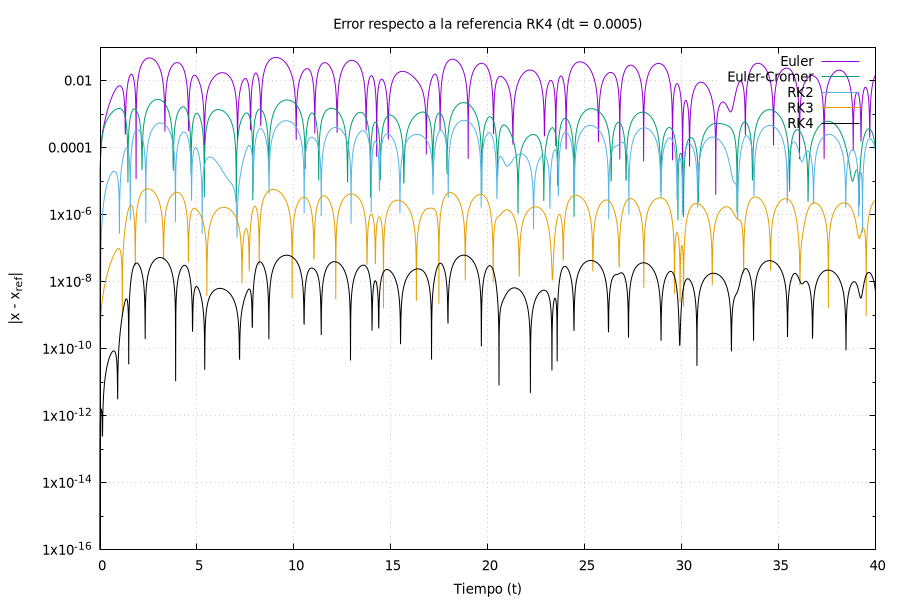
\includegraphics[width=0.78\textwidth]{error_vs_tiempo.png}
    \caption{Error $|x-x_{\mathrm{ref}}|$ en función del tiempo para los cinco métodos ($\Delta t=0.01$), frente a RK4 con $\Delta t=5\times10^{-4}$.}
    \label{fig:errt}
\end{figure}

\subsection{Transitorio y régimen estacionario (2d)}

Con $D=5$, $a=1$, $\gamma=0.2$, $A=2$ y $\omega=2$, el oscilador parte de $x_0=0.5$, $v_0=0$ y tarda unas decenas de unidades de tiempo en asentarse (Figura~\ref{fig:regimen}). A partir de $t\approx32$ los máximos de $x(t)$ quedan a menos de $5\times10^{-3}$ de su valor final. En el régimen estacionario:
\begin{itemize}
    \item $x(t)$ oscila entre $-0.378$ y $0.345$ con período $3.14\approx\pi=2\pi/\omega$: la respuesta es de período 1, igual al del forzamiento.
    \item La energía $E(t)$ oscila entre $0.29$ y $1.06$ sin deriva, porque la energía inyectada por el forzamiento se compensa con la disipada por el amortiguamiento a lo largo de cada ciclo.
    \item En el espacio de fase las trayectorias convergen a un ciclo límite cerrado.
\end{itemize}

\begin{figure}[H]
    \centering
    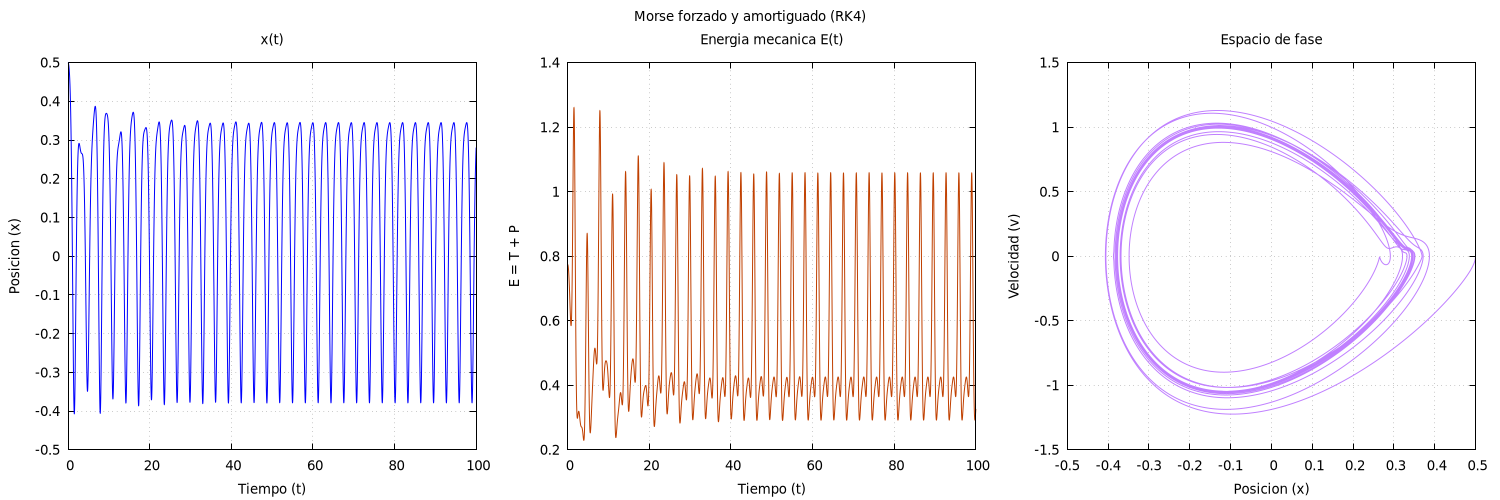
\includegraphics[width=\textwidth]{regimen_transitorio.png}
    \caption{Morse forzado y amortiguado con RK4 ($D=5$, $a=1$, $\gamma=0.2$, $A=2$, $\omega=2$): posición, energía mecánica y espacio de fase.}
    \label{fig:regimen}
\end{figure}

\subsection{Diagrama de bifurcación y exponente de Lyapunov (2e)}

La Tabla~\ref{tab:bif} resume lo que muestran, juntos, el diagrama de Poincaré (Figura~\ref{fig:bif}) y $\lambda_{\max}(A)$ (Figura~\ref{fig:lyap}). Los valores de $A$ son aproximados y se leyeron de los datos con paso $\Delta A=0.02$.

\begin{table}[H]
\centering
\small
\begin{tabular}{@{}p{3.1cm}p{4.2cm}p{6.2cm}@{}}
\toprule
Rango de $A$ & Respuesta (Poincaré) & $\lambda_{\max}$\\
\midrule
$1.5$ a $\approx2.05$ & Un punto (período $T$) & Promedio $-0.249$ hasta $A\approx1.9$; luego sube hacia 0\\
$\approx2.06$ & Primera duplicación de período & Se acerca a 0 ($-0.005$ en $A=2.06$)\\
$\approx2.08$ a $2.32$ & Dos puntos (período $2T$) & Negativo; un pico aislado $+0.082$ en $A=2.24$\\
$\approx2.36$ a $2.40$ & Cuatro puntos (período $4T$) & Cerca de 0 en $A=2.34$ ($-0.004$); negativo en $2.36$--$2.40$\\
$\gtrsim2.44$ & Nube de puntos (caos) & Positivo, crece hasta $\approx0.25$--$0.34$\\
$A=3.14$ & Ventana periódica & $-0.034$, único valor negativo para $A>2.5$\\
$2.6$ a $3.98$ & Banda caótica que se ensancha & Promedio $0.274$, máximo $0.343$ en $A=3.5$\\
\bottomrule
\end{tabular}
\caption{Regímenes dinámicos al variar la amplitud del forzamiento ($\gamma=0.5$, $\omega=2.6$).}
\label{tab:bif}
\end{table}

En ninguna de las 125 amplitudes se superó el umbral de disociación $x=15$, y el máximo de $x$ en los puntos de Poincaré fue $6.08$. El enlace oscila con grandes excursiones hacia la zona blanda del potencial, pero no se rompe.

\begin{figure}[H]
    \centering
    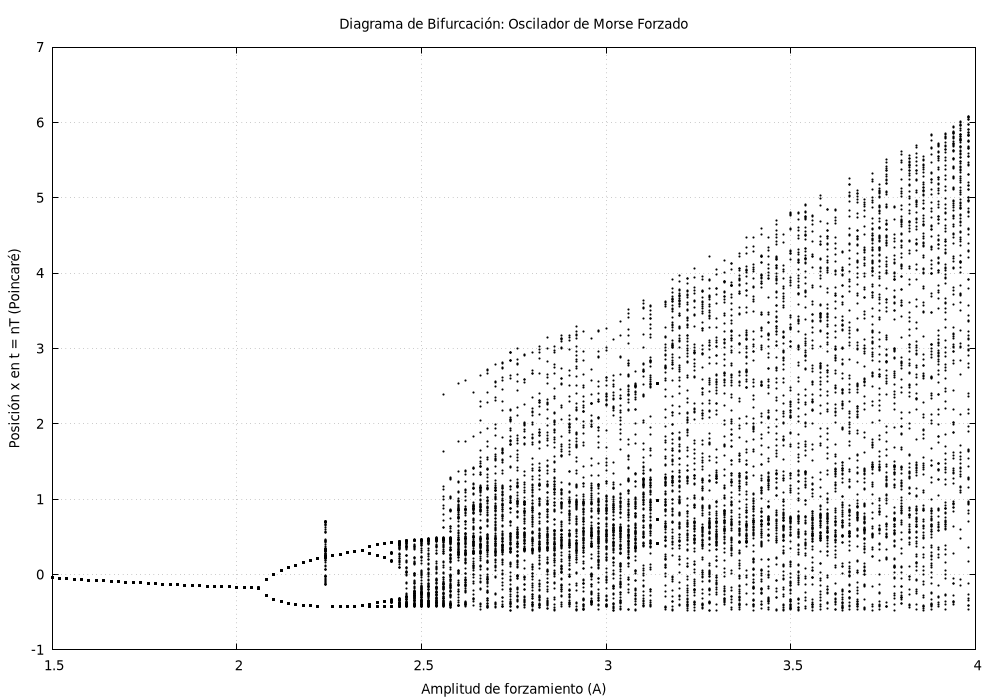
\includegraphics[width=0.85\textwidth]{diagrama_bifurcacion.png}
    \caption{Diagrama de bifurcación: posición en $t=nT$ frente a la amplitud $A$ ($\gamma=0.5$, $\omega=2.6$).}
    \label{fig:bif}
\end{figure}

\begin{figure}[H]
    \centering
    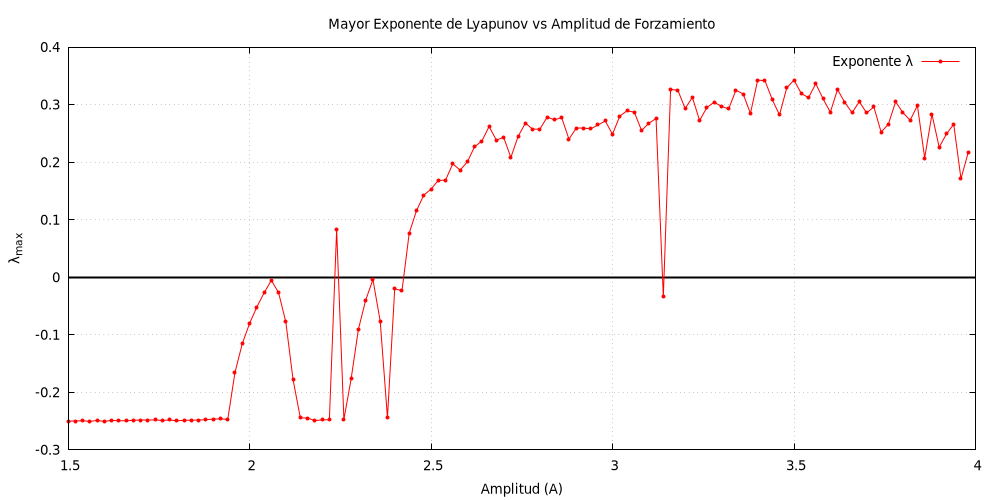
\includegraphics[width=0.85\textwidth]{lyapunov.png}
    \caption{Mayor exponente de Lyapunov frente a $A$. La línea negra marca $\lambda=0$.}
    \label{fig:lyap}
\end{figure}

\subsection{Osciladores acoplados (2f)}

Con $D=5$, $a=1$, $\gamma=0.5$, $A=3$, $\omega=2.6$ y $\kappa=1.5$, el oscilador 1 parte de $(0.5,\,0)$ y el 2 de $(0.501,\,0.5)$. A $A=3$ cada oscilador aislado es caótico ($\lambda_{\max}=0.25$ en la Figura~\ref{fig:lyap}), pero el par se sincroniza: el error $e(t)=|x_1-x_2|$ decae de forma aproximadamente exponencial (Tabla~\ref{tab:sync} y Figura~\ref{fig:sync}). El ajuste a la envolvente del error entre $t=10$ y $t=80$ da una tasa de decaimiento de $\approx0.22$ por unidad de tiempo ($e\propto \ee^{-0.22\,t}$).

\begin{table}[H]
\centering
\footnotesize
\setlength{\tabcolsep}{3pt}
\begin{tabular}{@{}lcccccccc@{}}
\toprule
$t$ & 0 & 1 & 5 & 10 & 20 & 40 & 60 & 80\\
\midrule
$e(t)$ & $1.0\times10^{-3}$ & $0.19$ & $0.13$ & $4.9\times10^{-2}$ & $2.1\times10^{-3}$ & $3.8\times10^{-5}$ & $2.0\times10^{-7}$ & $5.0\times10^{-9}$\\
\bottomrule
\end{tabular}
\caption{Error de sincronización en instantes seleccionados.}
\label{tab:sync}
\end{table}

\begin{figure}[H]
    \centering
    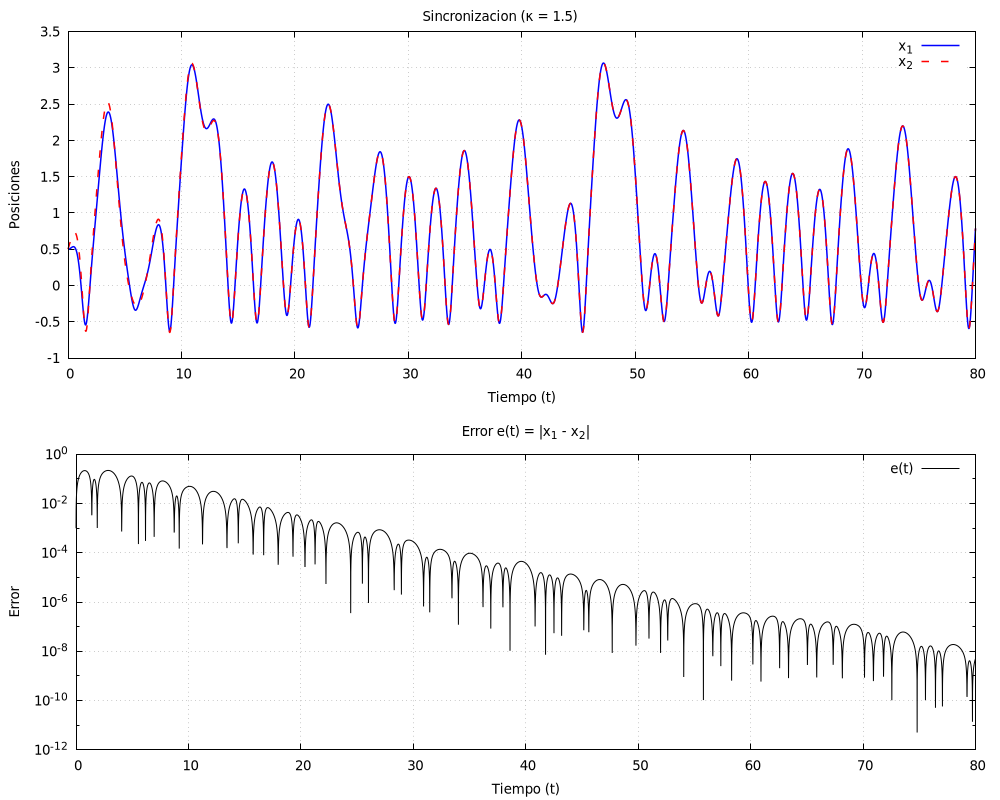
\includegraphics[width=0.85\textwidth]{sincronizacion_k_1.5.png}
    \caption{Sincronización con $\kappa=1.5$: posiciones $x_1(t)$ y $x_2(t)$ (arriba) y error $e(t)$ en escala logarítmica (abajo).}
    \label{fig:sync}
\end{figure}

\section{Discusión física y numérica}

\paragraph{Orden de los métodos.} Los órdenes observados (Tabla~\ref{tab:orden}) coinciden con los teóricos: $0.99$ y $1.07$ para los dos métodos de primer orden, $2.02$ para RK2, $3.00$ para RK3 y $4.07$ para RK4. Eso confirma que los cinco integradores están bien implementados y que, con estos pasos, el error está dominado por el truncamiento y no por el redondeo. Como el error de referencia (RK4 con $\Delta t=5\times10^{-4}$) escala como $\Delta t^{4}$, su valor estimado es del orden de $10^{-14}$; por eso los errores se pueden interpretar hasta aproximadamente $10^{-13}$.

\paragraph{Euler-Cromer frente a RK2.} Con pasos grandes Euler-Cromer tiene un error menor que RK2 (en $\Delta t=0.02$: $2.1\times10^{-4}$ contra $3.4\times10^{-4}$), pero al ser de primer orden pierde la ventaja al refinar el paso: ya en $\Delta t=0.01$ ambos son casi iguales y en $\Delta t=1.25\times10^{-3}$ RK2 es siete veces más preciso. Las curvas se cruzan en la Figura~\ref{fig:conv}. Además, el sistema es disipativo y forzado, así que la propiedad simpléctica de Euler-Cromer no se aprovecha.

\paragraph{Costo.} El tiempo crece más rápido que el número de evaluaciones de la fuerza: RK4 hace cuatro veces las evaluaciones de Euler pero tarda unas 13 veces más. No se investigó la causa (los tiempos dependen de la máquina y de las opciones de compilación). Aun así, la precisión se gana mucho más rápido que el costo: con $\Delta t=0.01$, RK4 es unas $3\times10^{6}$ veces más preciso que Euler a un costo unas 13 veces mayor. Para lograr con Euler un error de $5\times10^{-9}$ haría falta, por su orden 1, un paso unas $3\times10^{6}$ veces menor, es decir, del orden de $10^{10}$ pasos hasta $t=40$. Por eso RK4 es la elección razonable para este problema.

\paragraph{Validación física.} Con $\gamma=A=0$ el código reproduce los resultados exactos del oscilador de Morse: conservación de la energía, período dependiente de la energía (Tabla~\ref{tab:validacion}) y puntos de retorno. Esto valida la fuerza, el potencial y el integrador antes de añadir amortiguamiento y forzamiento.

\paragraph{Ruta al caos.} Al aumentar $A$ el sistema sigue una cascada de duplicación de período, $T\to2T\to4T$, hasta entrar en un régimen caótico, lo que es característico de osciladores no lineales forzados \cite{strogatz2015}. Los dos diagnósticos son consistentes: el exponente de Lyapunov se acerca a cero en cada bifurcación y se vuelve positivo donde el diagrama de Poincaré se llena de puntos. En el régimen periódico, $\lambda_{\max}\approx-0.249$ es muy cercano a $-\gamma/(2m)=-0.25$, el valor que corresponde a repartir por igual entre los dos exponentes la contracción total $-\gamma/m$ del espacio de fase. La ventana periódica de $A=3.14$ muestra que dentro de la zona caótica quedan intervalos regulares.

\paragraph{Sincronización.} Dos osciladores caóticos idénticos, con condiciones iniciales distintas, se sincronizan cuando el acoplamiento es suficientemente fuerte \cite{pecora1990}. Aquí $\kappa=1.5$ basta: el error decae unos siete órdenes de magnitud entre $t=10$ y $t=80$. La diferencia $\delta=x_1-x_2$ recibe además una fuerza restauradora $-(2\kappa/m)\,\delta$ que, junto con el amortiguamiento, tiende a anularla y compite con la divergencia propia de la dinámica caótica. La tasa medida ($\approx0.22$) es del mismo orden que $\gamma/(2m)=0.25$, lo que sugiere que la disipación controla el decaimiento; esto es solo una estimación y no se verificó con un análisis lineal.

\paragraph{Limitaciones.}
\begin{itemize}
    \item Cada valor de $A$ del diagrama de bifurcación arranca siempre de la misma condición inicial, $(0.5,\,0)$. No se barrió $A$ hacia arriba y hacia abajo, así que no se puede descartar la coexistencia de atractores (por ejemplo, el punto aislado en $A=2.24$) ni histéresis.
    \item $\lambda_{\max}$ se calcula con 300 períodos, y sus valores fluctúan de una amplitud a otra en la zona caótica (la Figura~\ref{fig:lyap} muestra variaciones de varias centésimas). Los valores del texto son indicativos, no precisos.
    \item Los experimentos de convergencia usan una sola condición inicial y un solo juego de parámetros.
    \item El valor de $\kappa$ para sincronizar se probó solo en $\kappa=1.5$; no se determinó el umbral mínimo.
\end{itemize}

\section{Conclusiones}

\begin{enumerate}[label=\textbf{\arabic*.}]
    \item Los cinco integradores alcanzan sus órdenes teóricos (observados: $0.99$, $1.07$, $2.02$, $3.00$ y $4.07$). RK4 es el más conveniente: con $\Delta t=0.01$ su error es $5.2\times10^{-9}$, frente a $1.5\times10^{-2}$ de Euler, a un costo unas 13 veces mayor.
    \item El código se valida con el caso conservativo: la energía se conserva y el período, los puntos de retorno y la velocidad máxima coinciden con las expresiones exactas del potencial de Morse.
    \item Con $\gamma=0.2$, $A=2$ y $\omega=2$, el oscilador alcanza en $t\approx32$ un ciclo límite de período $\pi$, igual al del forzamiento.
    \item Al variar $A$ (con $\gamma=0.5$, $\omega=2.6$) aparece una cascada de duplicación de período desde $A\approx2.06$ y caos desde $A\approx2.44$, con una ventana periódica en $A=3.14$. El exponente de Lyapunov y el diagrama de Poincaré concuerdan, y el enlace no se disocia en $1.5\le A\le4$.
    \item Dos osciladores caóticos idénticos ($A=3$) acoplados con $\kappa=1.5$ se sincronizan: el error llega a $0.19$ en $t\approx1$ y cae a $5\times10^{-9}$ en $t=80$.
\end{enumerate}

\begin{thebibliography}{9}
\bibitem{morse1929} P.~M. Morse, ``Diatomic molecules according to the wave mechanics. II. Vibrational levels'', \textit{Physical Review} \textbf{34}, 57--64 (1929).
\bibitem{cromer1981} A. Cromer, ``Stable solutions using the Euler approximation'', \textit{American Journal of Physics} \textbf{49}, 455--459 (1981).
\bibitem{press2007} W.~H. Press, S.~A. Teukolsky, W.~T. Vetterling y B.~P. Flannery, \textit{Numerical Recipes: The Art of Scientific Computing}, 3.ª ed., Cambridge University Press (2007).
\bibitem{benettin1980} G. Benettin, L. Galgani, A. Giorgilli y J.-M. Strelcyn, ``Lyapunov characteristic exponents for smooth dynamical systems and for Hamiltonian systems; a method for computing all of them. Part 1: Theory'', \textit{Meccanica} \textbf{15}, 9--20 (1980).
\bibitem{strogatz2015} S.~H. Strogatz, \textit{Nonlinear Dynamics and Chaos}, 2.ª ed., Westview Press (2015).
\bibitem{pecora1990} L.~M. Pecora y T.~L. Carroll, ``Synchronization in chaotic systems'', \textit{Physical Review Letters} \textbf{64}, 821--824 (1990).
\end{thebibliography}

\end{document}
